\documentclass[a0,portrait]{a0poster}

\usepackage{multicol}
\columnsep=100pt
\columnseprule=3pt

\usepackage[svgnames]{xcolor}

\usepackage{times}
\usepackage{palatino}

\usepackage{graphicx}
\graphicspath{{figures/}}
\usepackage{booktabs}
\usepackage[font=small,labelfont=bf]{caption}
\usepackage{amsfonts, amsmath, amsthm, amssymb}
\usepackage{wrapfig}
\usepackage{lipsum,adjustbox}
\usepackage[absolute,overlay]{textpos}
\usepackage{multirow}
\usepackage{titlesec}
\usepackage{url}
\usepackage{tikz}
\usepackage{tikz-dependency}
\usetikzlibrary{arrows.meta}
\captionsetup{labelformat=empty}

\begin{document}

\begin{center}
	\veryHuge \color{NavyBlue} \textbf{Multitask Parsing Across Semantic Representations}
\end{center}
\vspace{-1cm}
\begin{minipage}[b]{.07\linewidth}
\includegraphics[width=\linewidth]{huji_logo.jpg}
\vspace{5mm}
\end{minipage}
\begin{minipage}[b]{.16\linewidth}
\includegraphics[width=\linewidth]{huji_banner.png}
\includegraphics[width=\linewidth]{cse_banner.jpg}
\vspace{.8mm}
\end{minipage}
\hspace{1cm}
\begin{minipage}[b]{0.57\linewidth}
\LARGE \textbf{Daniel Hershcovich}\textsuperscript{1,2} \&
	   \textbf{Omri Abend}\textsuperscript{2} \&
	   \textbf{Ari Rappoport}\textsuperscript{2} \\[0.5cm] % Author(s)
\Large $^1$The Edmond and Lily Safra Center for Brain Sciences \\
  $^2$School of Computer Science and Engineering
  \setlength{\columnseprule}{0pt}
  \setlength\multicolsep{-20pt}
  \begin{multicols}{2}
  The Hebrew University of Jerusalem
  \large \texttt{\{danielh,oabend,arir\}@cs.huji.ac.il}
  \end{multicols}
\end{minipage}
\hfill
\begin{minipage}[b]{.09\linewidth}
\includegraphics[width=\linewidth]{elsc_logo.png}\vspace{5mm}
\includegraphics[width=\linewidth]{icrici_banner.png}
\end{minipage}

\vspace{1cm}
\titlespacing*{\section}{0pt}{8mm}{5mm}

%----------------------------------------------------------------------------------------

\begin{adjustbox}{margin=3mm,frame,minipage=.6\linewidth,center}
\Large\color{Navy}
Multitask learning allows a transition-based semantic parser
to generalize from multiple tasks,
improving UCCA parsing in challenging settings.
\end{adjustbox}


\begin{multicols}{2}


\color{Black}

\section*{Introduction}

\setlength{\columnsep}{1cm}

\begin{minipage}{.4\columnwidth}
  \begin{tikzpicture}[level distance=3cm, sibling distance=3cm, ->]
    \node (ROOT) [fill=black, circle] {}
      child {node (After) {After} edge from parent node[above] {\scriptsize $L$}}
      child {node (graduation) [fill=black, circle] {}
      {
        child {node {graduation} edge from parent node[left] {\scriptsize $P$}}
      } edge from parent node[left] {\scriptsize $H$} }
      child {node {,} edge from parent node[below] {\scriptsize $U$}}
      child {node (moved) [fill=black, circle] {}
      {
        child {node (John) {John} edge from parent node[left] {\scriptsize $A$}}
        child {node {moved} edge from parent node[left] {\scriptsize $P$}}
        child {node [fill=black, circle] {}
        {
          child {node {to} edge from parent node[left] {\scriptsize $R$}}
          child {node {Paris} edge from parent node[right] {\scriptsize $C$}}
        } edge from parent node[above] {\scriptsize $A$} }
      } edge from parent node[above] {\scriptsize $H$} }
      ;
    \draw[dashed,->] (graduation) to node [above] {\scriptsize $A$} (John);
    \node (LKG) at (-3,0) [fill=cyan, circle] {};
    \draw[bend right,color=cyan] (LKG) to node [auto, left] {\scriptsize $LR$} (After);
    \draw[color=cyan] (LKG) to[out=-60, in=190] node [below] {\scriptsize $LA\quad$} (graduation);
    \draw[color=cyan] (LKG) to[out=30, in=90] node [above] {\scriptsize $LA$} (moved);
  \end{tikzpicture}
  \captionof{figure}{UCCA}
  \end{minipage}
  
\begin{minipage}{.4\columnwidth}
  \begin{tikzpicture}[->,
      every node/.append style={sloped,anchor=south,auto=false,font=\tiny},
      level 1/.style={level distance=4cm,sibling distance=4cm},
      level 2/.style={level distance=4cm},
      level 3/.style={level distance=3cm}]
    \node (ROOT) [draw=black,ellipse] {move-01}
      child {node [draw=black,ellipse] {after}
      {
            child {node (graduation) [draw=black,ellipse] {graduate-01} edge from parent node {op1} }
      } edge from parent node {time} }
      child {node (John) [draw=black,ellipse] {person}
      {
        child {node [draw=black,ellipse] {name}
        {
            child {node [draw=black,ellipse] {"John"} edge from parent node {op1} }
        } edge from parent node {name} }
      } edge from parent node {ARG0} }
      child {node [draw=black,ellipse] {city}
      {
        child {node [draw=black,ellipse] {name}
        {
            child {node [draw=black,ellipse] {"Paris"} edge from parent node {op1} }
        } edge from parent node {name} }
      } edge from parent node {ARG2} }
      ;
      \draw (graduation) to node {ARG0} (John);
  \end{tikzpicture}
  \captionof{figure}{AMR}
\end{minipage}

    \begin{dependency}[text only label, label style={above}, font=\small]
    \begin{deptext}[column sep=.8em,ampersand replacement=\^]
    After \^ graduation \^ , \^ John \^ moved \^ to \^ Paris \\
    \end{deptext}
        \depedge[edge unit distance=1ex]{1}{2}{ARG2}
        \depedge[edge unit distance=1ex]{5}{4}{ARG1}
        \depedge[edge unit distance=1ex, edge end x offset=-2pt]{1}{5}{ARG1}
        \deproot[edge unit distance=1.5ex]{5}{top}
        \depedge[edge unit distance=2ex, edge start x offset=-1pt, edge end x offset=3pt]{5}{7}{ARG2}
        \depedge[edge unit distance=1ex, edge end x offset=5pt]{6}{5}{ARG1}
        \depedge[edge unit distance=1ex]{6}{7}{ARG2}
    \end{dependency}
  \captionof{figure}{DM}

    \begin{dependency}[text only label, label style={above}, font=\small]
    \begin{deptext}[column sep=.8em,ampersand replacement=\^]
    After \^ graduation \^ , \^ John \^ moved \^ to \^ Paris \\
    \end{deptext}
        \depedge[edge unit distance=1ex]{2}{1}{case}
        \depedge[edge unit distance=1ex]{4}{3}{punct}
        \depedge[edge unit distance=1ex]{5}{4}{nsubj}
        \depedge[edge unit distance=1ex, edge end x offset=-2pt]{2}{5}{obl}
        \depedge[edge unit distance=1ex]{7}{6}{case}
        \deproot[edge unit distance=1.5ex]{5}{root}
        \depedge[edge unit distance=1.5ex]{5}{7}{obl}
    \end{dependency}
  \captionof{figure}{UD}


\rule{\columnwidth}{1pt}

\section*{Transition-based UCCA Parsing}

TUPA{}, our transition-based parser, supports the structural properties of UCCA.

Transition-based parsers work by applying a \textit{transition}
at each step to the parser state,
defined using a buffer $B$ of tokens and nodes to be processed,
a stack $S$ of nodes currently being processed,
and a graph $G=(V,E,\ell)$ of constructed nodes and edges.

\scalebox{.9}{
\begin{minipage}{.55\columnwidth}
	\begin{tikzpicture}[level distance=22mm, sibling distance=4cm]
	\draw[color=gray,dashed] (.2,-.2) rectangle (19.5,2.7);
	\draw[color=gray] (.4,0) rectangle (2.6,1);
	\node[anchor=west] at (1,2) {$S$};
	\node[fill=black, circle] at (1.5,.45) {};
	\draw[color=gray] (3,0) rectangle (17,1);
	\node[anchor=west] at (10,2) {$B$};
	\node[anchor=west] at (3,.45) {\small After graduation , John moved to Paris .};
	\node[anchor=west] at (18,2) {$G$};
	\node[fill=black, circle] at (18.5,.45) {};
	\node[anchor=west] at (10,-.8) {\small\textsc{Shift}};
	\draw[arrows={->[line width=2pt,length=4mm,width=6mm]}] (9,-.2) -- (9,-1.4);
	\end{tikzpicture}
	\begin{tikzpicture}[level distance=22mm, sibling distance=4cm]
	\draw[color=gray,dashed] (.2,-.2) rectangle (19.5,2.7);
	\draw[color=gray] (.4,0) rectangle (4.3,1);
	\node[anchor=west] at (1,2) {$S$};
	\node[fill=black, circle] at (1.5,.45) {};
	\node[color=red,anchor=west] at (2,.45) {\small After};
	\draw[color=gray] (5,0) rectangle (17,1);
	\node[anchor=west] at (10,2) {$B$};
	\node[anchor=west] at (5,.45) {\small graduation , John moved to Paris .};
	\node[anchor=west] at (18,2) {$G$};
	\node[fill=black, circle] at (18.5,.45) {};
	\node[anchor=west] at (10,-.9) {\small\textsc{Right-Edge\textsubscript L}};
	\draw[arrows={->[line width=2pt,length=4mm,width=6mm]}] (9,-.2) -- (9,-1.4);
	\end{tikzpicture}
	\begin{tikzpicture}[level distance=22mm, sibling distance=4cm]
	\draw[color=gray,dashed] (.2,-.6) rectangle (19.5,2.7);
	\draw[color=gray] (.4,0) rectangle (4.3,1);
	\node[anchor=west] at (1,2) {$S$};
	\node[fill=black, circle] at (1.5,.45) {};
	\node[anchor=west] at (2,.45) {\small After};
	\draw[color=gray] (5,0) rectangle (17,1);
	\node[anchor=west] at (10,2) {$B$};
	\node[anchor=west] at (5,.45) {\small graduation , John moved to Paris .};
	\node[anchor=west] at (16.5,2) {$G$};
	\node[fill=black, circle] at (18.5,2.2) {}
	  child {node  {\scriptsize After} edge from parent [-{Latex[length=4mm]},red] node[left] {\small L}};
	\node[anchor=west] at (10,-1.2) {\small\textsc{Reduce}};
	\draw[arrows={->[line width=2pt,length=4mm,width=6mm]}] (9,-.6) -- (9,-1.7);
	\end{tikzpicture}
	\begin{tikzpicture}[level distance=22mm, sibling distance=4cm]
	\draw[color=gray,dashed] (.2,-.6) rectangle (19.5,2.7);
	\draw[color=gray] (.4,0) rectangle (3,1);
	\node[anchor=west] at (1,2) {$S$};
	\node[fill=black, circle] at (1.5,.45) {};
	\draw[color=gray] (5,0) rectangle (17,1);
	\node[anchor=west] at (10,2) {$B$};
	\node[anchor=west] at (5,.45) {\small graduation , John moved to Paris .};
	\node[anchor=west] at (16.5,2) {$G$};
	\node[fill=black, circle] at (18.5,2.2) {}
	  child {node  {\scriptsize After} edge from parent [-{Latex[length=4mm]}] node[left] {\small L}};
	\node[anchor=west] at (10,-1.2) {\small\textsc{Shift}};
	\draw[arrows={->[line width=2pt,length=4mm,width=6mm]}] (9,-.6) -- (9,-1.7);
	\end{tikzpicture}
	\begin{tikzpicture}[level distance=22mm, sibling distance=4cm]
	\draw[color=gray,dashed] (.2,-.6) rectangle (19.5,2.7);
	\draw[color=gray] (.4,0) rectangle (6,1);
	\node[anchor=west] at (1,2) {$S$};
	\node[fill=black, circle] at (1.5,.45) {};
	\node[color=red,anchor=west] at (2,.45) {\small graduation};
	\draw[color=gray] (8.5,0) rectangle (17,1);
	\node[anchor=west] at (10,2) {$B$};
	\node[anchor=west] at (8.8,.45) {\small , John moved to Paris .};
	\node[anchor=west] at (16.5,2) {$G$};
	\node[fill=black, circle] at (18.5,2.2) {}
	  child {node  {\scriptsize After} edge from parent [-{Latex[length=4mm]}] node[left] {\small L}};
	\node[anchor=west] at (10,-1.2) {\small\textsc{Node\textsubscript P}};
	\draw[arrows={->[line width=2pt,length=4mm,width=6mm]}] (9,-.6) -- (9,-1.7);
	\end{tikzpicture}
	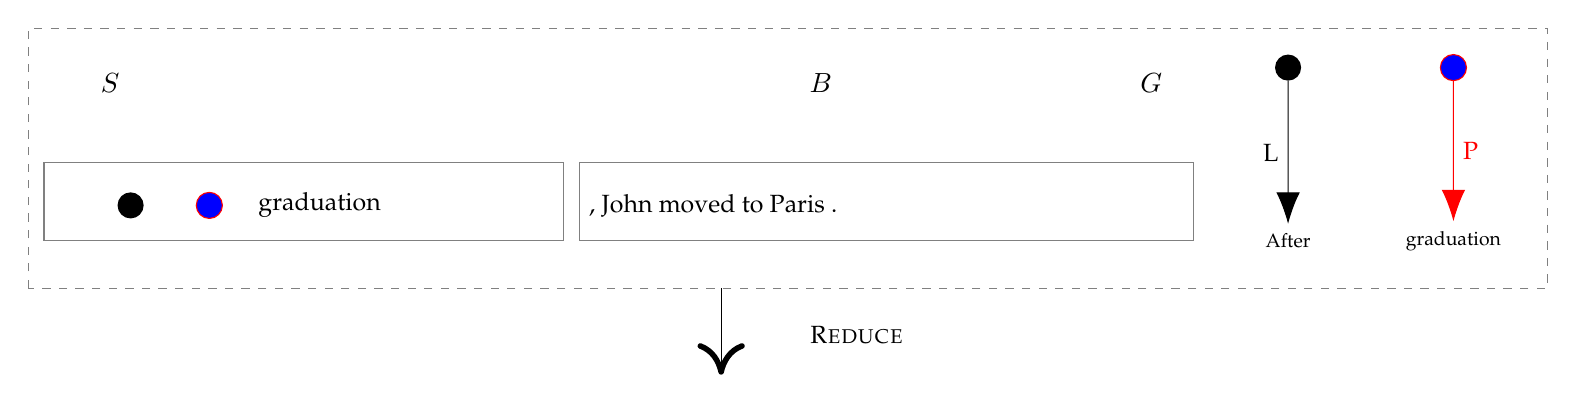
\begin{tikzpicture}[level distance=22mm, sibling distance=4cm]
	\draw[color=gray,dashed] (.2,-.6) rectangle (19.5,2.7);
	\draw[color=gray] (.4,0) rectangle (7,1);
	\node[anchor=west] at (1,2) {$S$};
	\node[fill=black, circle] at (1.5,.45) {};
	\node[fill=blue, draw=red, circle] at (2.5,.45) {};
	\node[anchor=west] at (3,.45) {\small graduation};
	\draw[color=gray] (7.2,0) rectangle (15,1);
	\node[anchor=west] at (10,2) {$B$};
	\node[anchor=west] at (7.2,.45) {\small , John moved to Paris .};
	\node[anchor=west] at (14.2,2) {$G$};
	\node[fill=black, circle] at (16.2,2.2) {}
	  child {node  {\scriptsize After} edge from parent [-{Latex[length=4mm]}] node[left] {\small L}};
	\node[fill=blue, draw=red, circle] at (18.3,2.2) {}
	  child {node {\scriptsize graduation} edge from parent [-{Latex[length=4mm]},red] node[right] {\small P}};
	\node[anchor=west] at (10,-1.2) {\small\textsc{Reduce}};
	\draw[arrows={->[line width=2pt,length=4mm,width=6mm]}] (9,-.6) -- (9,-1.7);
	\end{tikzpicture}
\end{minipage}
\hspace{1cm}
\begin{minipage}{.4\columnwidth}
	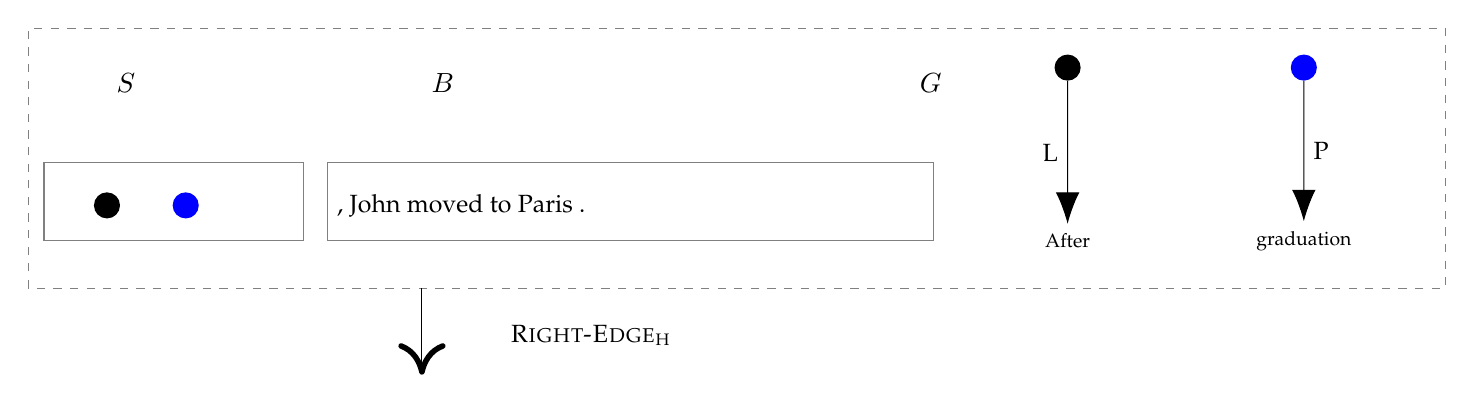
\begin{tikzpicture}[level distance=22mm, sibling distance=4cm]
	\draw[color=gray,dashed] (0,-.6) rectangle (18,2.7);
	\draw[color=gray] (0.2,0) rectangle (3.5,1);
	\node[anchor=west] at (1,2) {$S$};
	\node[fill=black, circle] at (1,.45) {};
	\node[fill=blue, circle] at (2,.45) {};
	\draw[color=gray] (3.8,0) rectangle (11.5,1);
	\node[anchor=west] at (5,2) {$B$};
	\node[anchor=west] at (3.8,.45) {\small , John moved to Paris .};
	\node[anchor=west] at (11.2,2) {$G$};
	\node[fill=black, circle] at (13.2,2.2) {}
	  child {node  {\scriptsize After} edge from parent [-{Latex[length=4mm]}] node[left] {\small L}};
	\node[fill=blue, circle] at (16.2,2.2) {}
	  child {node {\scriptsize graduation} edge from parent [-{Latex[length=4mm]}] node[right] {\small P}};
	\node[anchor=west] at (6,-1.2) {\small\textsc{Right-Edge\textsubscript H}};
	\draw[arrows={->[line width=2pt,length=4mm,width=6mm]}] (5,-.6) -- (5,-1.7);
	\end{tikzpicture}
	\begin{tikzpicture}[level distance=22mm, sibling distance=4cm]
	\draw[color=gray,dashed] (0,-3.2) rectangle (18,2.7);
	\draw[color=gray] (0.2,0) rectangle (3.5,1);
	\node[anchor=west] at (1,2) {$S$};
	\node[fill=black, circle] at (1,.45) {};
	\node[fill=blue, circle] at (2,.45) {};
	\draw[color=gray] (3.8,0) rectangle (11.5,1);
	\node[anchor=west] at (5,2) {$B$};
	\node[anchor=west] at (3.8,.45) {\small , John moved to Paris .};
	\node[anchor=west] at (12,2) {$G$};
	\node[fill=black, circle] at (14.7,1.5) {}
	  child {node  {\scriptsize After} edge from parent [-{Latex[length=4mm]}] node[left] {\small L}}
	  child {node [fill=blue, circle] {}
	  {
	    child {node {\scriptsize graduation} edge from parent [-{Latex[length=4mm]},black] node[right] {\small P}}
	  } edge from parent [-{Latex[length=5mm]},red] node[right] {\small H} };
	\node[anchor=west] at (6,-3.6) {\small\textsc{Shift}};
	\draw[arrows={->[line width=2pt,length=4mm,width=6mm]}] (5,-3.2) -- (5,-4.3);
	\end{tikzpicture}
	\begin{tikzpicture}[level distance=22mm, sibling distance=4cm]
	\draw[color=gray,dashed] (0,-3.2) rectangle (18,2.7);
	\draw[color=gray] (0.2,0) rectangle (3.6,1);
	\node[anchor=west] at (1,2) {$S$};
	\node[fill=black, circle] at (1,.45) {};
	\node[fill=blue, circle] at (2,.45) {};
	\node[color=red, anchor=west] at (3,.25) {\small ,};
	\draw[color=gray] (3.9,0) rectangle (11.5,1);
	\node[anchor=west] at (5,2) {$B$};
	\node[anchor=west] at (3.9,.45) {\small John moved to Paris .};
	\node[anchor=west] at (12,2) {$G$};
	\node[fill=black, circle] at (14.7,1.5) {}
	  child {node  {\scriptsize After} edge from parent [-{Latex[length=4mm]}] node[left] {\small L}}
	  child {node [fill=blue, circle] {}
	  {
	    child {node {\scriptsize graduation} edge from parent [-{Latex[length=4mm]}] node[right] {\small P}}
	  } edge from parent [-{Latex[length=5mm]}] node[right] {\small H} };
	\node[anchor=west] at (6,-3.9) {\Large \ldots};
	\draw[arrows={->[line width=2pt,length=4mm,width=6mm]}] (5,-3.2) -- (5,-4.3);
	\end{tikzpicture}
	\begin{tikzpicture}[level distance=22mm, sibling distance=3cm]
	\draw[color=gray,dashed] (0,-5.5) rectangle (18,2.7);
	\draw[color=gray] (.2,0) rectangle (.9,1);
	\node[anchor=west] at (0,2) {$S$};
	\draw[color=gray] (1.3,0) rectangle (2.1,1);
	\node[anchor=west] at (1,2) {$B$};
	\node[anchor=west] at (3,2) {$G$};
    \node (ROOT) [fill=black,circle] at (8,1.5) {}
      child {node (After) {\scriptsize After} edge from parent node[left] {\small L}}
      child {node (graduation) [fill=blue,circle] {}
      {
        child {node {\scriptsize graduation} edge from parent node[left] {\small P}}
      } edge from parent node[left] {\small H} }
      child {node {\scriptsize ,} edge from parent node[right] {\small U}}
      child {node (moved) [fill=purple,circle] {}
      {
        child {node (John) {\scriptsize John} edge from parent node[left] {\small A}}
        child {node {\scriptsize moved} edge from parent node[left] {\small P}}
        child {node [fill=orange,circle] {}
        {
          child {node {\scriptsize to} edge from parent node[left] {\small R}}
          child {node {\scriptsize Paris} edge from parent node[right] {\small C}}
        } edge from parent node[right] {\small A} }
      } edge from parent node[right] {\small H} }
      ;
    \draw[dashed,-{Latex[length=5mm]}] (graduation) to node [auto] {\small A} (John);
	\end{tikzpicture}
\end{minipage}
}
\captionof{figure}{Example for intermediate states during transition-based UCCA parsing.}
\vspace{5mm}

A classifier selects the next transition based on the current state's features.
It is trained by an oracle based on gold-standard annotations.
We experiment with three classifiers:
\begin{flushleft}
	\begin{tabular}{ll}
	\textbf{TUPA{Sparse}} & Perceptron with features: words, POS, dependency \& edge label combinations. \\
	\textbf{TUPA{MLP}} & 2-layer NN, learned embedding features + external word embeddings. \\
	\textbf{TUPA{BiLSTM}} & 2-layer bidirectional RNN to encode features, 2-layer NN for classification. \\
	\end{tabular}
\end{flushleft}
\vspace{5mm}
For all classifiers, inference is performed greedily, i.e., without beam search.

Parser code available at \url{https://github.com/danielhers/tupa}\\
All corpora available at \url{http://www.cs.huji.ac.il/~oabend/ucca.html}\\
Parser written in Python using DyNet: \url{https://github.com/clab/dynet}

\begin{center}
    \begin{tikzpicture}[level distance=3cm, sibling distance=4cm, ->,
        every circle node/.append style={fill=black}]
      \tikzstyle{word} = [font=\rmfamily,color=black]
      \node (ROOT) [circle] {}
        child {node (After) [word] {After} edge from parent node[above] {\scriptsize $L$}}
        child {node (graduation) [circle] {}
        {
          child {node [word] {graduation} edge from parent node[left] {\scriptsize $P$}}
        } edge from parent node[right] {\scriptsize $H$} }
        child {node [word] {,} edge from parent node[below] {\scriptsize $U$}}
        child {node (moved) [circle] {}
        {
          child {node (John) [word] {John} edge from parent node[left] {\scriptsize $A$}}
          child {node [word] {moved} edge from parent node[left] {\scriptsize $P$}}
          child {node [circle] {}
          {
            child {node [word] {to} edge from parent node[left] {\scriptsize $R$}}
            child {node [word] {Paris} edge from parent node[right] {\scriptsize $C$}}
          } edge from parent node[above] {\scriptsize $A$} }
        } edge from parent node[right] {\scriptsize $H$} }
        ;
      \draw[dashed,->] (graduation) to node [above] {\scriptsize $A$} (John);
    \end{tikzpicture}
  \caption{UCCA}
  
  \begin{tikzpicture}[level distance=4cm, ->,
      every node/.append style={sloped,anchor=south,auto=false,font=\scriptsize},
      level 1/.style={sibling distance=6cm},
      level 2/.style={sibling distance=3cm},
      level 3/.style={sibling distance=3cm}]
    \tikzstyle{word} = [font=\rmfamily,color=black]
    \node (ROOT) [word] {moved}
      child {node [word] {After}
      {
            child {node (graduation) [word] {graduation} edge from parent node {op} }
      } edge from parent node {time} }
      child {node (John) [fill=black,circle] {}
      {
        child {node [word] {John} edge from parent node {name} }
      } edge from parent node {ARG0} }
      child {node [fill=black,circle] {}
      {
        child {node [word] {Paris} edge from parent node {name} }
      } edge from parent node {ARG2} }
      ;
      \draw[dashed] (graduation) to node {ARG0} (John);
  \end{tikzpicture}
  \captionof{figure}{AMR}

  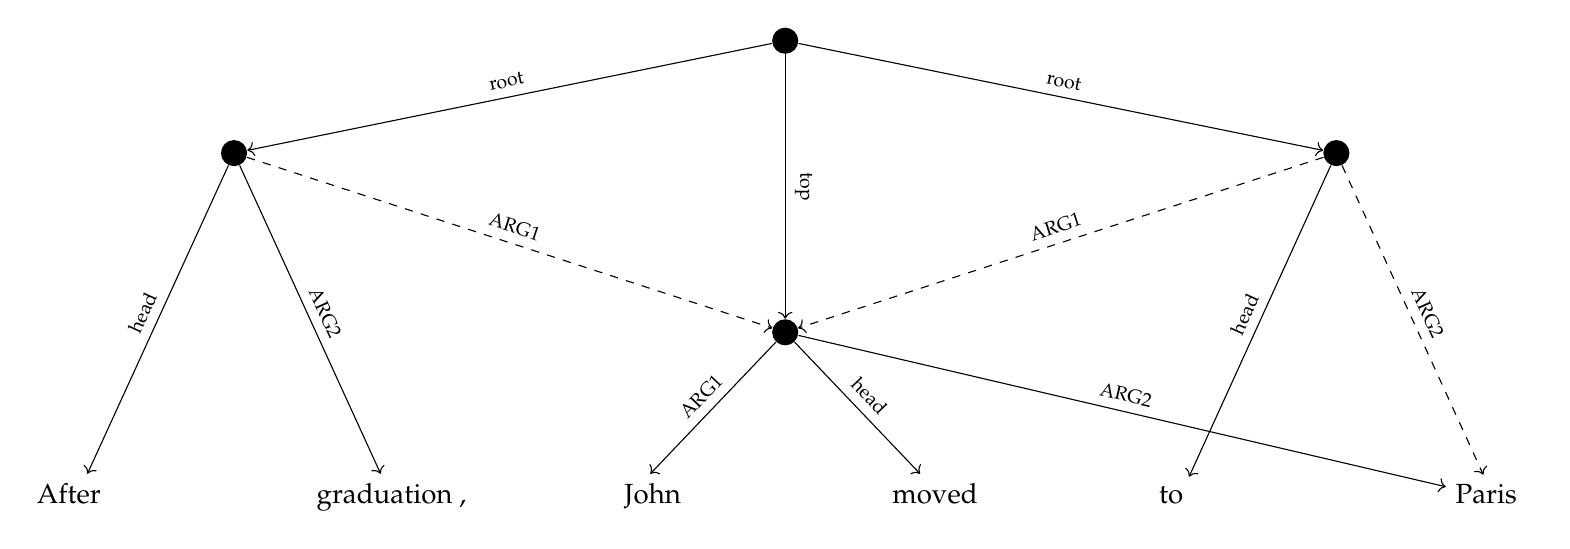
\begin{tikzpicture}[level distance=22mm, ->,
      every node/.append style={sloped,anchor=south,auto=false,font=\scriptsize},
      level 1/.style={sibling distance=7cm,level distance=16mm},
      level 2/.style={sibling distance=4cm,level distance=24mm}]
    \tikzstyle{word} = [font=\rmfamily,color=black]
    \node (ROOT) [fill=black,circle] {}
      child {node (after) [fill=black,circle] {}
      {
        child {node [draw=none] {}
        {
          child {node [word] (after_word) {After{\color{white}g}} edge from parent [draw=none]}
        } edge from parent [draw=none] }
        child {node [draw=none] {}
        {
          child {node [word] (graduation) {graduation ,} edge from parent [draw=none]}
        } edge from parent [draw=none] }
      } edge from parent node {root}}
      child {node [draw=none] {}
      {
        child {node (moved) [fill=black,circle] {}
        {
          child {node [word] {\quad{\color{white}g} John} edge from parent node {ARG1}}
          child {node [word] {moved{\color{white}g}} edge from parent node {head}}
        } edge from parent [draw=none] }
      } edge from parent [draw=none] }
      child {node (to) [fill=black,circle] {}
      {
        child {node [draw=none] {}
        {
            child {node [word] (to_word) {to{\color{white}g}} edge from parent [draw=none]}
          } edge from parent [draw=none] }
          child {node [draw=none] {}
        {
          child {node [word] (Paris) {Paris{\color{white}g}} edge from parent [draw=none]}
        } edge from parent [draw=none] }
      } edge from parent node {root}}
      ;
      \draw (ROOT) to node {top} (moved);
      \draw (after) to node {head} (after_word);
      \draw (after) to node {ARG2} (graduation);
      \draw[dashed] (after) to node {ARG1} (moved);
      \draw[dashed] (to) to node {ARG1} (moved);
      \draw (to) to node {head} (to_word);
      \draw (moved) to node {ARG2} (Paris);
      \draw[dashed] (to) to node {ARG2} (Paris);
  \end{tikzpicture}
  \captionof{figure}{DM}

  \begin{tikzpicture}[level distance=3cm, ->,
      every node/.append style={sloped,anchor=south,auto=false,font=\scriptsize},
      level 1/.style={sibling distance=4cm},
      level 2/.style={sibling distance=3cm}]
    \tikzstyle{word} = [font=\rmfamily,color=black]
    \node (ROOT) [fill=black,circle] {}
      child {node (after) [fill=black,circle] {}
      {
        child {node [word] {After{\color{white}g}\quad\quad} edge from parent node {case}}
        child {node [word] {\quad graduation\quad\quad} edge from parent node {head}}
      } edge from parent node {obl}}
      child {node {}
      {
        child {node [word] (comma) {\quad,{\color{white}g}} edge from parent [draw=none]}
      } edge from parent [draw=none]}
      child {node {}
      {
        child {node [word] (John) {John{\color{white}g}} edge from parent [draw=none]}
      } edge from parent [draw=none]}
      child {node {}
      {
        child {node [word] (moved) {moved{\color{white}g}} edge from parent [draw=none]}
      } edge from parent [draw=none]}
      child {node (to) [fill=black,circle] {}
      {
          child {node [word] {to{\color{white}g}} edge from parent node {case}}
          child {node [word] {Paris{\color{white}g}} edge from parent node {head}}
      } edge from parent node {obl}}
      ;
      \draw (ROOT) to node {punct} (comma);
      \draw (ROOT) to node {nsubj} (John);
      \draw (ROOT) to node {head} (moved);
  \end{tikzpicture}
  \captionof{figure}{UD}
\end{center}

\section*{Experimental Setup}

\paragraph{Corpora.}
English Wikipedia (in-domain), English part of \textit{Twenty Thousand Leagues Under the Sea}
English-French parallel corpus (out-of-domain).

\paragraph{Evaluation.}
Labeled precision, recall and F-score on graph edges,
represented by their terminal yields.
Primary and remote evaluated separately.

\paragraph{Baselines.}
Parsers trained on bilexical graphs and trees converted from UCCA training set,
and evaluated by converting test set output to UCCA.

\begin{wrapfigure}{l}{.6\columnwidth}
	\vspace{-5cm}
	\centering
	\begin{dependency}[theme = simple]
	\begin{deptext}[column sep=.7em,ampersand replacement=\^]
	After \^ graduation \^ , \^ John \^ moved \^ to \^ Paris \\
	\end{deptext}
		\depedge{2}{1}{L}
		\depedge{2}{3}{U}
		\depedge[dashed]{2}{4}{A}
		\depedge{5}{4}{A}
		\depedge{2}{5}{H}
		\depedge{7}{6}{R}
		\depedge{5}{7}{A}
	\end{dependency}
	\begin{dependency}[theme = simple]
	\begin{deptext}[column sep=.7em,ampersand replacement=\^]
	John \^ gave \^ everything \^ up \\
	\end{deptext}
		\depedge{2}{1}{A}
		\depedge{2}{3}{A}
		\depedge{2}{4}{C}
	\end{dependency}
	\begin{dependency}[theme = simple]
	\begin{deptext}[column sep=.7em,ampersand replacement=\^]
	John \^ and \^ Mary \^ went \^ home \\
	\end{deptext}
		\depedge[edge start x offset=-6pt]{1}{4}{A}
		\depedge{1}{2}{N}
		\depedge{1}{3}{C}
		\depedge{4}{5}{A}
	\end{dependency}
	\captionof{figure}{Bilexical graph approximation.}
\end{wrapfigure}

\vspace{5cm}

As no direct comparison with existing parsers is possible,
we compare TUPA{} to bilexical dependency graph parsers,
which support reentrancy and discontinuity but not non-terminal nodes.
We also convert UCCA to (bilexical) trees
and evaluate constituency and dependency tree parsers on them,
by simply removing remote edges from the graph.


\rule{\columnwidth}{1pt}



\section*{Results}

TUPA{BiLSTM} obtains the highest F-scores in all metrics:
	  
\begin{center}
	\begin{tabular}{l|ccc|ccc||ccc|ccc}
		& \multicolumn{6}{c||}{Wiki (in-domain)} & \multicolumn{6}{c}{20K Leagues (out-of-domain)} \\
		& \multicolumn{3}{c|}{Primary} & \multicolumn{3}{c||}{Remote}
		& \multicolumn{3}{c|}{Primary} & \multicolumn{3}{c}{Remote} \\
		& \textbf{LP} & \textbf{LR} & \textbf{LF} & \textbf{LP} & \textbf{LR} & \textbf{LF}
		& \textbf{LP} & \textbf{LR} & \textbf{LF} & \textbf{LP} & \textbf{LR} & \textbf{LF} \\
		\hline
		TUPA{Sparse}
		& 64.5 & 63.7 & 64.1 & 19.8 & 13.4 & 16
		& 59.6 & 59.9 & 59.8 & 22.2 & 7.7 & 11.5 \\
		%TUPA{Dense} 
		%& 59.1 & 58.9 & 59 & 17.4 & 12.4 & 14.5
		%& 57.0 & 57.9 & 57.4 & 10.8 & 4.2 & 6.0 \\
		TUPA{MLP}
		& 65.2 & 64.6 & 64.9 & 23.7 & 13.2 & 16.9
		& 62.3 & 62.6 & 62.5 & 20.9 & 6.3 & 9.7 \\
		TUPA{BiLSTM}
		& 74.4 & 72.7 & \textbf{73.5} & 47.4 & 51.6 & \textbf{49.4}
		& 68.7 & 68.5 & \textbf{68.6} & 38.6 & 18.8 & \textbf{25.3} \\
		\hline
		\multicolumn{8}{l}{\rule{0pt}{2ex} \footnotesize
		Bilexical Approximation (Dependency DAG Parsers)} \\
		\small Upper Bound
		%& \small 94.5 & \small 87.7 & \small 91 & \small 77.3 & \small 46.8 & \small 58.3
		%& \small 94.8 & \small 88 & \small 91.3 & \small 66.3 & \small 32.3 & \small 43.4 \\
		& & & \small 91 & & & \small 58.3
		& & & \small 91.3 & & & \small 43.4 \\
		DAGParser \cite{ribeyre-villemontedelaclergerie-seddah:2014:SemEval}
		& 61.8 & 55.8 & 58.6 & 9.5 & 0.5 & 1
		& 56.4 & 50.6 & 53.4 & -- & 0 & 0 \\
		TurboParser \cite{almeida-martins:2015:SemEval}
		& 57.7 & 46 & 51.2 & 77.8 & 1.8 & 3.7
		& 50.3 & 37.7 & 43.1 & 100 & 0.4 & 0.8 \\
		\hline
		\multicolumn{8}{l}{\rule{0pt}{2ex} \footnotesize
		Tree Approximation (Constituency Tree Parser)} \\
		\small Upper Bound
		%& \small 100 & \small 100 & \small 100 & & &
		%& \small 100 & \small 100 & \small 100 \\
		& & & \small 100 & & & \small --
		& & & \small 100 & & & \small -- \\
		\textsc{uparse} \cite{maier-lichte:2016:DiscoNLP}
		& 60.9 & 61.2 & 61.1 & -- & -- & --
		& 52.7 & 52.8 & 52.8 & -- & -- & -- \\
		\hline
		\multicolumn{8}{l}{\rule{0pt}{2ex} \footnotesize
		Bilexical Tree Approximation (Dependency Tree Parsers)} \\
		\small Upper Bound
		%& \small 94.5 & \small 87.7 & \small 91 & & &
		%& \small 94.8 & \small 88 & \small 91.3 \\
		& & & \small 91 & & & \small --
		& & & \small 91.3 & & & \small -- \\
		MaltParser \cite{nivre2007maltparser}
		& 62.8 & 57.7 & 60.2 & -- & -- & --
		& 57.8 & 53 & 55.3 & -- & -- & -- \\
		LSTM Parser \cite{dyer2015transition}
		& 73.2 & 66.9 & 69.9 & -- & -- & --
		& 66.1 & 61.1 & 63.5 & -- & -- & --
	\end{tabular}
\end{center}

The performance is encouraging in light of UCCA's inter-annotator agreement of 80--85\%
F-score on primary edges \cite{abend2013universal}.


\rule{\columnwidth}{1pt}


\begin{wrapfigure}{l}{18cm}
	\vspace{-1cm}
	\begin{tikzpicture}[level distance=22mm, sibling distance=4cm]
	\node[anchor=west] at (0,3.3) {Parser state};
	\draw[color=gray,dashed] (0,-3.2) rectangle (18,2.7);
	\draw[color=gray] (0.2,0) rectangle (3.6,1);
	\node[anchor=west] at (1,2) {$S$};
	\node[fill=black, circle] at (1,.45) {};
	\node[fill=blue, circle] at (2,.45) {};
	\node[anchor=west] at (3,.25) {\small ,};
	\draw[color=gray] (3.9,0) rectangle (11.5,1);
	\node[anchor=west] at (5,2) {$B$};
	\node[anchor=west] at (3.9,.45) {\small John moved to Paris .};
	\node[anchor=west] at (12,2) {$G$};
	\node[fill=black, circle] at (14.7,1.5) {}
	  child {node  {\scriptsize After} edge from parent [-{Latex[length=4mm]}] node[left] {\small L}}
	  child {node [fill=blue, circle] {}
	  {
	    child {node {\scriptsize graduation} edge from parent [-{Latex[length=4mm]}] node[right] {\small P}}
	  } edge from parent [-{Latex[length=5mm]}] node[right] {\small H} };
	\end{tikzpicture}
	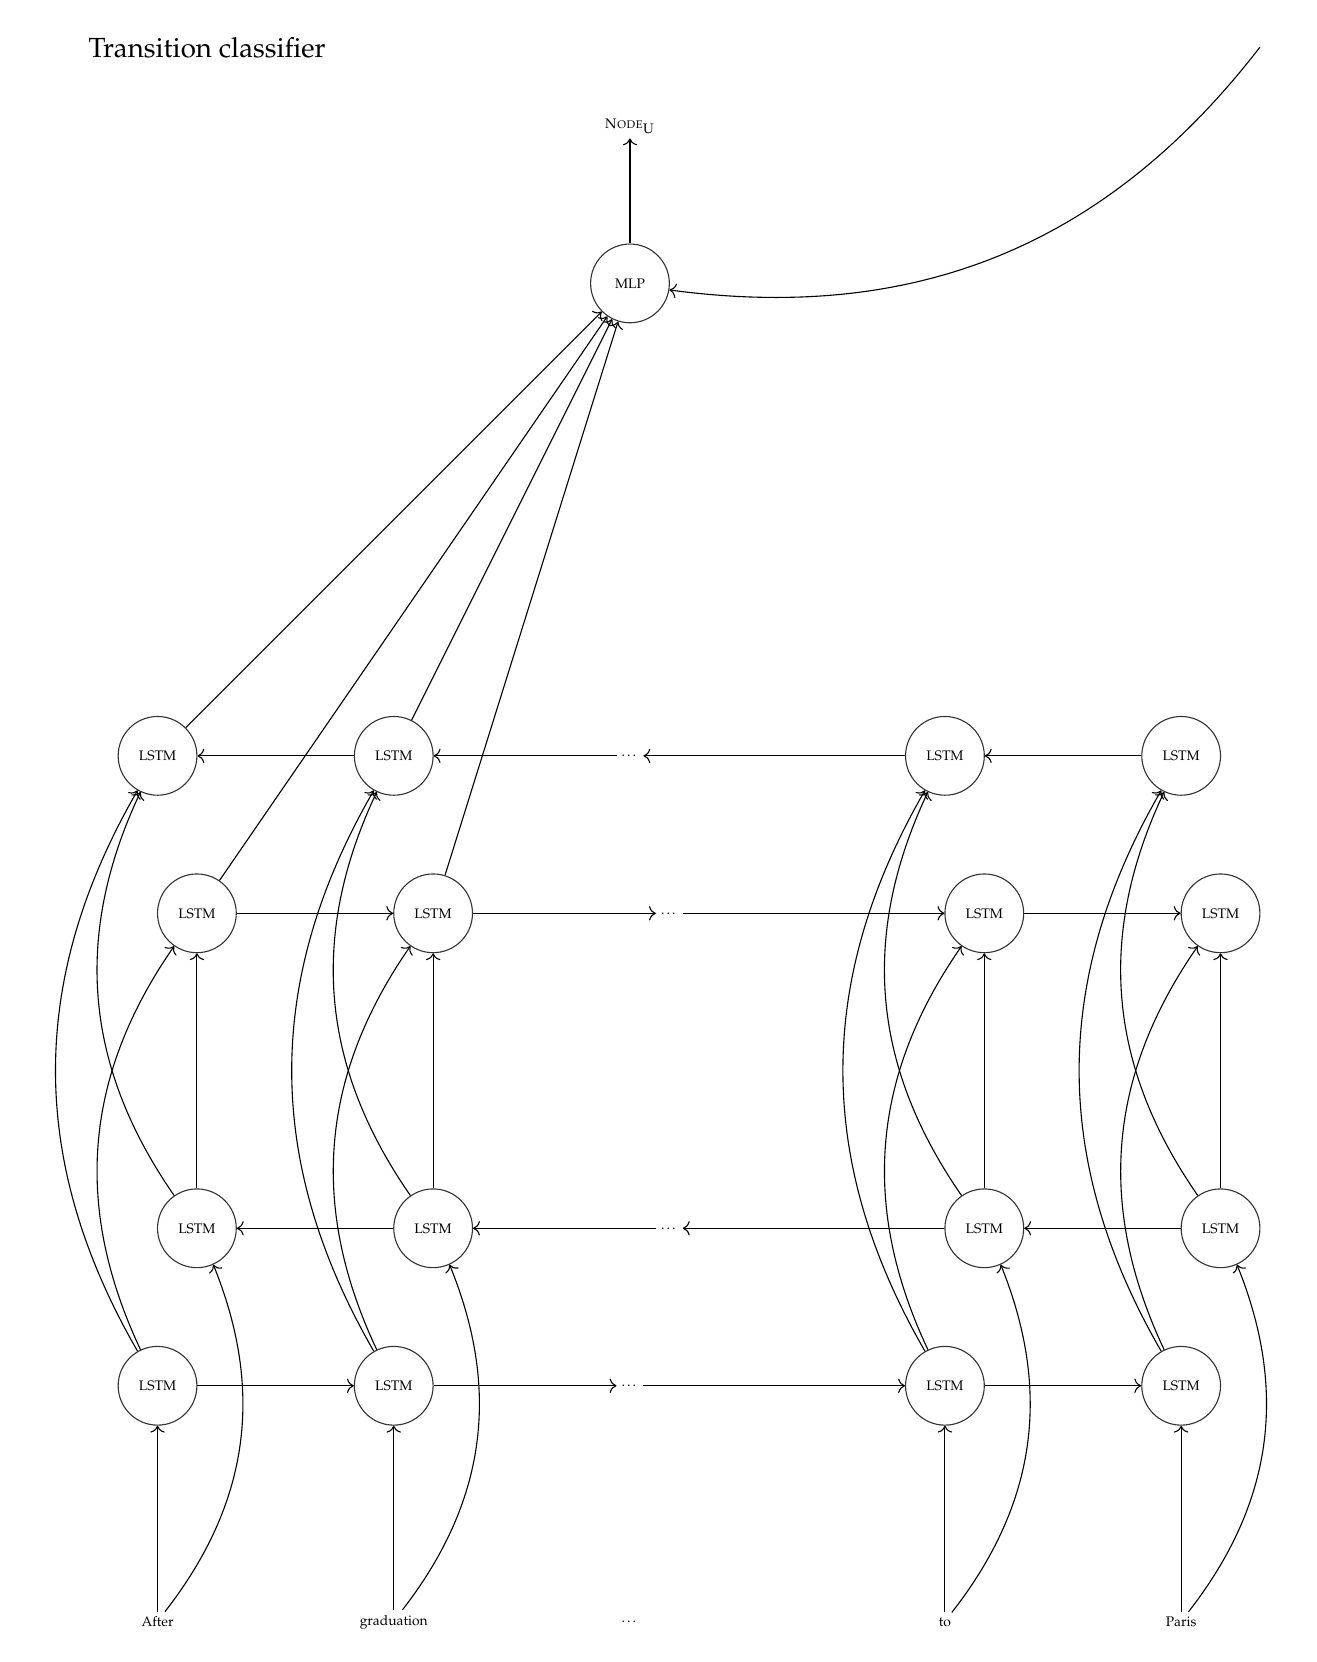
\begin{tikzpicture}[->]
	\node[anchor=west] at (0,17) {Transition classifier};
	\tiny
	\tikzstyle{main}=[circle, minimum size=1cm, draw=black!80, node distance=24mm]
	\foreach \i/\word in {1/{After},4/{graduation},11/{to},14/{Paris}} {
	    \node (x\i) at (\i,-3) {\word};
	    \node[main, fill=white!100] (h\i) at (\i,0) {LSTM};
        \path (x\i) edge (h\i);
	    \node[main, fill=white!100] (i\i) at (\i.5,2) {LSTM};
        \path (x\i) edge [bend right] (i\i);
	    \node[main, fill=white!100] (l\i) at (\i.5,6) {LSTM};
        \path (h\i) edge [bend left] (l\i);
        \path (i\i) edge (l\i);
	    \node[main, fill=white!100] (k\i) at (\i,8) {LSTM};
        \path (i\i) edge [bend left] (k\i);
        \path (h\i) edge [bend left] (k\i);
	}
    \node (k7) at (7,8) {\ldots};
    \node (l7) at (7.5,6) {\ldots};
    \node (i7) at (7.5,2) {\ldots};
    \node (h7) at (7,0) {\ldots};
    \node (x7) at (7,-3) {\ldots};
	\foreach \current/\next in {1/4,4/7,7/11,11/14} {
        \path (i\next) edge (i\current);
        \path (h\current) edge (h\next);
        \path (k\next) edge (k\current);
        \path (l\current) edge (l\next);
	}
    \node[main, fill=white!100] (mlp) at (7,14) {MLP};
	\foreach \i in {1,4} {
        \path (l\i) edge (mlp);
        \path (k\i) edge (mlp);
    }
    \coordinate (state) at (15,17);
    \path (state) edge [bend left] (mlp);
    \node (transition) at (7,16) {\textsc{Node}\textsubscript{U}};
    \path (mlp) edge (transition);
	\end{tikzpicture}
	\caption{Illustration of the TUPA{} model.}
\end{wrapfigure}

\section*{Conclusions}

We present TUPA{}, the first parser for UCCA, and show that with a
NN classifier and BiLSTM feature extractor,
it accurately predicts UCCA graphs from text, outperforming various
strong baselines.

Future work will explore different target representations,
and apply the parser to more languages,
demonstrating the importance of broad-coverage parsing.
A parser for UCCA will enable using the framework for new tasks.


\color{DarkSlateGray} % Set the color back to DarkSlateGray for the rest of the content
\tiny
%\nocite{*} % Print all references regardless of whether they were cited in the poster or not
\bibliographystyle{plain} % Plain referencing style
\bibliography{references}

\end{multicols}
\end{document}
